\documentclass[]{article}
\usepackage{lmodern}
\usepackage{amssymb,amsmath}
\usepackage{ifxetex,ifluatex}
\usepackage{fixltx2e} % provides \textsubscript
\ifnum 0\ifxetex 1\fi\ifluatex 1\fi=0 % if pdftex
  \usepackage[T1]{fontenc}
  \usepackage[utf8]{inputenc}
\else % if luatex or xelatex
  \ifxetex
    \usepackage{mathspec}
  \else
    \usepackage{fontspec}
  \fi
  \defaultfontfeatures{Ligatures=TeX,Scale=MatchLowercase}
\fi
% use upquote if available, for straight quotes in verbatim environments
\IfFileExists{upquote.sty}{\usepackage{upquote}}{}
% use microtype if available
\IfFileExists{microtype.sty}{%
\usepackage{microtype}
\UseMicrotypeSet[protrusion]{basicmath} % disable protrusion for tt fonts
}{}
\usepackage[margin=1in]{geometry}
\usepackage{hyperref}
\hypersetup{unicode=true,
            pdfborder={0 0 0},
            breaklinks=true}
\urlstyle{same}  % don't use monospace font for urls
\usepackage{color}
\usepackage{fancyvrb}
\newcommand{\VerbBar}{|}
\newcommand{\VERB}{\Verb[commandchars=\\\{\}]}
\DefineVerbatimEnvironment{Highlighting}{Verbatim}{commandchars=\\\{\}}
% Add ',fontsize=\small' for more characters per line
\usepackage{framed}
\definecolor{shadecolor}{RGB}{248,248,248}
\newenvironment{Shaded}{\begin{snugshade}}{\end{snugshade}}
\newcommand{\AlertTok}[1]{\textcolor[rgb]{0.94,0.16,0.16}{#1}}
\newcommand{\AnnotationTok}[1]{\textcolor[rgb]{0.56,0.35,0.01}{\textbf{\textit{#1}}}}
\newcommand{\AttributeTok}[1]{\textcolor[rgb]{0.77,0.63,0.00}{#1}}
\newcommand{\BaseNTok}[1]{\textcolor[rgb]{0.00,0.00,0.81}{#1}}
\newcommand{\BuiltInTok}[1]{#1}
\newcommand{\CharTok}[1]{\textcolor[rgb]{0.31,0.60,0.02}{#1}}
\newcommand{\CommentTok}[1]{\textcolor[rgb]{0.56,0.35,0.01}{\textit{#1}}}
\newcommand{\CommentVarTok}[1]{\textcolor[rgb]{0.56,0.35,0.01}{\textbf{\textit{#1}}}}
\newcommand{\ConstantTok}[1]{\textcolor[rgb]{0.00,0.00,0.00}{#1}}
\newcommand{\ControlFlowTok}[1]{\textcolor[rgb]{0.13,0.29,0.53}{\textbf{#1}}}
\newcommand{\DataTypeTok}[1]{\textcolor[rgb]{0.13,0.29,0.53}{#1}}
\newcommand{\DecValTok}[1]{\textcolor[rgb]{0.00,0.00,0.81}{#1}}
\newcommand{\DocumentationTok}[1]{\textcolor[rgb]{0.56,0.35,0.01}{\textbf{\textit{#1}}}}
\newcommand{\ErrorTok}[1]{\textcolor[rgb]{0.64,0.00,0.00}{\textbf{#1}}}
\newcommand{\ExtensionTok}[1]{#1}
\newcommand{\FloatTok}[1]{\textcolor[rgb]{0.00,0.00,0.81}{#1}}
\newcommand{\FunctionTok}[1]{\textcolor[rgb]{0.00,0.00,0.00}{#1}}
\newcommand{\ImportTok}[1]{#1}
\newcommand{\InformationTok}[1]{\textcolor[rgb]{0.56,0.35,0.01}{\textbf{\textit{#1}}}}
\newcommand{\KeywordTok}[1]{\textcolor[rgb]{0.13,0.29,0.53}{\textbf{#1}}}
\newcommand{\NormalTok}[1]{#1}
\newcommand{\OperatorTok}[1]{\textcolor[rgb]{0.81,0.36,0.00}{\textbf{#1}}}
\newcommand{\OtherTok}[1]{\textcolor[rgb]{0.56,0.35,0.01}{#1}}
\newcommand{\PreprocessorTok}[1]{\textcolor[rgb]{0.56,0.35,0.01}{\textit{#1}}}
\newcommand{\RegionMarkerTok}[1]{#1}
\newcommand{\SpecialCharTok}[1]{\textcolor[rgb]{0.00,0.00,0.00}{#1}}
\newcommand{\SpecialStringTok}[1]{\textcolor[rgb]{0.31,0.60,0.02}{#1}}
\newcommand{\StringTok}[1]{\textcolor[rgb]{0.31,0.60,0.02}{#1}}
\newcommand{\VariableTok}[1]{\textcolor[rgb]{0.00,0.00,0.00}{#1}}
\newcommand{\VerbatimStringTok}[1]{\textcolor[rgb]{0.31,0.60,0.02}{#1}}
\newcommand{\WarningTok}[1]{\textcolor[rgb]{0.56,0.35,0.01}{\textbf{\textit{#1}}}}
\usepackage{graphicx,grffile}
\makeatletter
\def\maxwidth{\ifdim\Gin@nat@width>\linewidth\linewidth\else\Gin@nat@width\fi}
\def\maxheight{\ifdim\Gin@nat@height>\textheight\textheight\else\Gin@nat@height\fi}
\makeatother
% Scale images if necessary, so that they will not overflow the page
% margins by default, and it is still possible to overwrite the defaults
% using explicit options in \includegraphics[width, height, ...]{}
\setkeys{Gin}{width=\maxwidth,height=\maxheight,keepaspectratio}
\IfFileExists{parskip.sty}{%
\usepackage{parskip}
}{% else
\setlength{\parindent}{0pt}
\setlength{\parskip}{6pt plus 2pt minus 1pt}
}
\setlength{\emergencystretch}{3em}  % prevent overfull lines
\providecommand{\tightlist}{%
  \setlength{\itemsep}{0pt}\setlength{\parskip}{0pt}}
\setcounter{secnumdepth}{0}
% Redefines (sub)paragraphs to behave more like sections
\ifx\paragraph\undefined\else
\let\oldparagraph\paragraph
\renewcommand{\paragraph}[1]{\oldparagraph{#1}\mbox{}}
\fi
\ifx\subparagraph\undefined\else
\let\oldsubparagraph\subparagraph
\renewcommand{\subparagraph}[1]{\oldsubparagraph{#1}\mbox{}}
\fi

%%% Use protect on footnotes to avoid problems with footnotes in titles
\let\rmarkdownfootnote\footnote%
\def\footnote{\protect\rmarkdownfootnote}

%%% Change title format to be more compact
\usepackage{titling}

% Create subtitle command for use in maketitle
\providecommand{\subtitle}[1]{
  \posttitle{
    \begin{center}\large#1\end{center}
    }
}

\setlength{\droptitle}{-2em}

  \title{}
    \pretitle{\vspace{\droptitle}}
  \posttitle{}
    \author{}
    \preauthor{}\postauthor{}
    \date{}
    \predate{}\postdate{}
  

\begin{document}

\hypertarget{regression-and-model-validation}{%
\section{Regression and model
validation}\label{regression-and-model-validation}}

\begin{itemize}
\tightlist
\item
  This week week I am doing regression analysis and model validation.
  But first I had to wrangle with the original data. That was pretty
  difficult for me. But finally with lots of errors and trying again I
  succeeded.*
\end{itemize}

\hypertarget{description-of-the-dataset}{%
\section{Description of the dataset}\label{description-of-the-dataset}}

\begin{Shaded}
\begin{Highlighting}[]
\NormalTok{students2014<-}\KeywordTok{read.csv}\NormalTok{(}\StringTok{"learning2014.csv"}\NormalTok{, }\DataTypeTok{header =} \OtherTok{TRUE}\NormalTok{, }\DataTypeTok{sep=} \StringTok{","}\NormalTok{)}

\CommentTok{# Looking at the structure}

\KeywordTok{str}\NormalTok{(students2014)}
\end{Highlighting}
\end{Shaded}

\begin{verbatim}
## 'data.frame':    166 obs. of  7 variables:
##  $ gender  : Factor w/ 2 levels "F","M": 1 2 1 2 2 1 2 1 2 1 ...
##  $ Age     : int  53 55 49 53 49 38 50 37 37 42 ...
##  $ Attitude: int  37 31 25 35 37 38 35 29 38 21 ...
##  $ deep    : num  3.58 2.92 3.5 3.5 3.67 ...
##  $ stra    : num  3.38 2.75 3.62 3.12 3.62 ...
##  $ surf    : num  2.58 3.17 2.25 2.25 2.83 ...
##  $ Points  : int  25 12 24 10 22 21 21 31 24 26 ...
\end{verbatim}

\begin{Shaded}
\begin{Highlighting}[]
\KeywordTok{head}\NormalTok{(students2014)}
\end{Highlighting}
\end{Shaded}

\begin{verbatim}
##   gender Age Attitude     deep  stra     surf Points
## 1      F  53       37 3.583333 3.375 2.583333     25
## 2      M  55       31 2.916667 2.750 3.166667     12
## 3      F  49       25 3.500000 3.625 2.250000     24
## 4      M  53       35 3.500000 3.125 2.250000     10
## 5      M  49       37 3.666667 3.625 2.833333     22
## 6      F  38       38 4.750000 3.625 2.416667     21
\end{verbatim}

This data has 166 observations which means 166 students. This data has 7
variables. The 7 variables are gender, age, attitude, deep, stra, surf
and points. The attitude variable gives information of the students'
global attitude toward statistics. Points mean exam points and their
points related to different aspects of learning (Deep, strategic and
surface learning).

\hypertarget{show-graphical-overview-of-the-data-and-show-summaries-of-variables-in-the-data}{%
\subsection{Show graphical overview of the data and show summaries of
variables in the
data}\label{show-graphical-overview-of-the-data-and-show-summaries-of-variables-in-the-data}}

\begin{Shaded}
\begin{Highlighting}[]
\KeywordTok{pairs}\NormalTok{(students2014[}\OperatorTok{-}\DecValTok{1}\NormalTok{], }\DataTypeTok{col=}\NormalTok{students2014}\OperatorTok{$}\NormalTok{gender)}
\end{Highlighting}
\end{Shaded}

\includegraphics{chapter2_files/figure-latex/unnamed-chunk-2-1.pdf}

\begin{Shaded}
\begin{Highlighting}[]
\KeywordTok{summary}\NormalTok{(students2014)}
\end{Highlighting}
\end{Shaded}

\begin{verbatim}
##  gender       Age           Attitude          deep            stra      
##  F:110   Min.   :17.00   Min.   :14.00   Min.   :1.583   Min.   :1.250  
##  M: 56   1st Qu.:21.00   1st Qu.:26.00   1st Qu.:3.333   1st Qu.:2.625  
##          Median :22.00   Median :32.00   Median :3.667   Median :3.188  
##          Mean   :25.51   Mean   :31.43   Mean   :3.680   Mean   :3.121  
##          3rd Qu.:27.00   3rd Qu.:37.00   3rd Qu.:4.083   3rd Qu.:3.625  
##          Max.   :55.00   Max.   :50.00   Max.   :4.917   Max.   :5.000  
##       surf           Points     
##  Min.   :1.583   Min.   : 7.00  
##  1st Qu.:2.417   1st Qu.:19.00  
##  Median :2.833   Median :23.00  
##  Mean   :2.787   Mean   :22.72  
##  3rd Qu.:3.167   3rd Qu.:27.75  
##  Max.   :4.333   Max.   :33.00
\end{verbatim}

This picture is not actually helping me to understand what kind of data
I am prosessing. I like the summarize table and actually I use it quite
often when getting familiar with my data. Let's look at it more closely.

\begin{Shaded}
\begin{Highlighting}[]
\KeywordTok{summary}\NormalTok{(students2014)}
\end{Highlighting}
\end{Shaded}

\begin{verbatim}
##  gender       Age           Attitude          deep            stra      
##  F:110   Min.   :17.00   Min.   :14.00   Min.   :1.583   Min.   :1.250  
##  M: 56   1st Qu.:21.00   1st Qu.:26.00   1st Qu.:3.333   1st Qu.:2.625  
##          Median :22.00   Median :32.00   Median :3.667   Median :3.188  
##          Mean   :25.51   Mean   :31.43   Mean   :3.680   Mean   :3.121  
##          3rd Qu.:27.00   3rd Qu.:37.00   3rd Qu.:4.083   3rd Qu.:3.625  
##          Max.   :55.00   Max.   :50.00   Max.   :4.917   Max.   :5.000  
##       surf           Points     
##  Min.   :1.583   Min.   : 7.00  
##  1st Qu.:2.417   1st Qu.:19.00  
##  Median :2.833   Median :23.00  
##  Mean   :2.787   Mean   :22.72  
##  3rd Qu.:3.167   3rd Qu.:27.75  
##  Max.   :4.333   Max.   :33.00
\end{verbatim}

There are 110 females and 56 males. Minimum age is 17, median 22, mean
25.51, maximum 55. There are also quartiles you can use; 1st quartile
21, 3rd quartile 27. Exam points are minimum 7, median 23, mean 22.72,
maximum 33.0, 1st quartile 19, 3rd quartile 27.75. Global attitude
minimum 14, median 32, mean 31.43, max 50, 1st quartile 26, 3rd quartile
37. Deep questions points minimum 1.58, median 3.667, mean 3.68, 3rd
quartile 4.083. And so on. Not everybody like these kinds of table but
for me it gives quick insight into my data and I use it quite often.

\hypertarget{use-the-packages-ggally-and-ggplot2-and-get-some-help-with-the-graphical-overview}{%
\section{Use the packages GGally and ggplot2 and get some help with the
graphical
overview}\label{use-the-packages-ggally-and-ggplot2-and-get-some-help-with-the-graphical-overview}}

\begin{Shaded}
\begin{Highlighting}[]
\KeywordTok{library}\NormalTok{(GGally)}
\end{Highlighting}
\end{Shaded}

\begin{verbatim}
## Loading required package: ggplot2
\end{verbatim}

\begin{verbatim}
## Registered S3 method overwritten by 'GGally':
##   method from   
##   +.gg   ggplot2
\end{verbatim}

\begin{Shaded}
\begin{Highlighting}[]
\KeywordTok{library}\NormalTok{(ggplot2)}

\NormalTok{p <-}\StringTok{ }\KeywordTok{ggpairs}\NormalTok{(students2014, }\DataTypeTok{mapping =} \KeywordTok{aes}\NormalTok{(}\DataTypeTok{alpha=}\FloatTok{0.5}\NormalTok{), }\DataTypeTok{lower =} \KeywordTok{list}\NormalTok{(}\DataTypeTok{combo =} \KeywordTok{wrap}\NormalTok{(}\StringTok{"facethist"}\NormalTok{, }\DataTypeTok{bins =} \DecValTok{20}\NormalTok{)))}

\NormalTok{p}
\end{Highlighting}
\end{Shaded}

\includegraphics{chapter2_files/figure-latex/unnamed-chunk-4-1.pdf}

This way the data is more easily readable. Almost all the variables are
normally distributes. The age is skewed. The picture also shows that
there is not a very strong correlation between different variables since
the correlations are between -0.3 - 0.4.

\hypertarget{choose-three-variables-as-explanatory-variables-and-fit-a-regression-model-where-exam-points-is-the-target-dependent-variable.}{%
\subsection{Choose three variables as explanatory variables and fit a
regression model where exam points is the target (dependent)
variable.}\label{choose-three-variables-as-explanatory-variables-and-fit-a-regression-model-where-exam-points-is-the-target-dependent-variable.}}

\begin{Shaded}
\begin{Highlighting}[]
\NormalTok{model <-}\StringTok{ }\KeywordTok{lm}\NormalTok{(Points }\OperatorTok{~}\StringTok{ }\NormalTok{gender }\OperatorTok{+}\StringTok{ }\NormalTok{Attitude }\OperatorTok{+}\StringTok{ }\NormalTok{stra, }\DataTypeTok{data =}\NormalTok{ students2014)}
\KeywordTok{summary}\NormalTok{(model)}
\end{Highlighting}
\end{Shaded}

\begin{verbatim}
## 
## Call:
## lm(formula = Points ~ gender + Attitude + stra, data = students2014)
## 
## Residuals:
##      Min       1Q   Median       3Q      Max 
## -17.7179  -3.3285   0.5343   3.7412  10.9007 
## 
## Coefficients:
##             Estimate Std. Error t value Pr(>|t|)    
## (Intercept)  8.97982    2.40303   3.737 0.000258 ***
## genderM     -0.22362    0.92477  -0.242 0.809231    
## Attitude     0.35100    0.05956   5.893 2.13e-08 ***
## stra         0.89107    0.54409   1.638 0.103419    
## ---
## Signif. codes:  0 '***' 0.001 '**' 0.01 '*' 0.05 '.' 0.1 ' ' 1
## 
## Residual standard error: 5.304 on 162 degrees of freedom
## Multiple R-squared:  0.2051, Adjusted R-squared:  0.1904 
## F-statistic: 13.93 on 3 and 162 DF,  p-value: 3.982e-08
\end{verbatim}

This test studied the association of exam points (target value, which
was asked) with gender, attitude and strategic learning (explanatory
variables). It can be seen that the Attitude is the only value that is
statistically siginificant (p-value is \textless{} 0.05.). Actually the
p-value is very low.

\hypertarget{next-we-are-using-a-summary-of-my-fitted-model-to-explain-the-relationship-between-the-chosen-explanatory-variable-and-the-target-variable.}{%
\subsection{Next we are using a summary of my fitted model, to explain
the relationship between the chosen explanatory variable and the target
variable.}\label{next-we-are-using-a-summary-of-my-fitted-model-to-explain-the-relationship-between-the-chosen-explanatory-variable-and-the-target-variable.}}

\textbf{I am doing a regression model of with the one significant
explanatory variable ``Attitude''. }

\begin{Shaded}
\begin{Highlighting}[]
\NormalTok{model_}\DecValTok{2}\NormalTok{ <-}\StringTok{ }\KeywordTok{lm}\NormalTok{(Points }\OperatorTok{~}\StringTok{ }\NormalTok{Attitude, }\DataTypeTok{data =}\NormalTok{ students2014)}
\KeywordTok{summary}\NormalTok{(model_}\DecValTok{2}\NormalTok{)}
\end{Highlighting}
\end{Shaded}

\begin{verbatim}
## 
## Call:
## lm(formula = Points ~ Attitude, data = students2014)
## 
## Residuals:
##      Min       1Q   Median       3Q      Max 
## -16.9763  -3.2119   0.4339   4.1534  10.6645 
## 
## Coefficients:
##             Estimate Std. Error t value Pr(>|t|)    
## (Intercept) 11.63715    1.83035   6.358 1.95e-09 ***
## Attitude     0.35255    0.05674   6.214 4.12e-09 ***
## ---
## Signif. codes:  0 '***' 0.001 '**' 0.01 '*' 0.05 '.' 0.1 ' ' 1
## 
## Residual standard error: 5.32 on 164 degrees of freedom
## Multiple R-squared:  0.1906, Adjusted R-squared:  0.1856 
## F-statistic: 38.61 on 1 and 164 DF,  p-value: 4.119e-09
\end{verbatim}

\#These results mean that the attitude's estimate is 0.35 and the
p-value stays still \textless{}0.05 being statistically significant. In
other words this means that when the attitude increases by 1 unit the
exam points increase by 0.35.

\hypertarget{exlaining-the-the-multiple-r-squared-of-the-model.}{%
\subsection{Exlaining the the multiple R squared of the
model.}\label{exlaining-the-the-multiple-r-squared-of-the-model.}}

R-squared is a statistical method showing how close the data is to the
fitted regression line. Meaning how well does the model fit to my data.
In general it can be said that the higher the R-squared, the better the
model fits to the data. The definition of R-squared is the percentage of
the response variable variation that is explained by a linear
model.R-squared = Explained variation / Total variation R-squared, it is
always between 0 and 100\%. In this summary we can see that the multiple
R-squared is 0.1906 so 19\% which means that this model explains only
1/5 of the exam points around their mean. R-squared does not determine
whether the coefficient estimates and predictions are biased. This is
why you must assess the residual plots.

\hypertarget{produce-the-following-diagnostic-plots-residuals-vs-fitted-values-normal-qq-plot-and-residuals-vs-leverage.}{%
\subsection{Produce the following diagnostic plots: Residuals vs Fitted
values, Normal QQ-plot and Residuals vs
Leverage.}\label{produce-the-following-diagnostic-plots-residuals-vs-fitted-values-normal-qq-plot-and-residuals-vs-leverage.}}

There are several assumptions in the linear regression model. With the
help of these plots you can analyze the residuals of the model and see
how well the linear regression model is working or are the some problems
with it.

\begin{Shaded}
\begin{Highlighting}[]
\KeywordTok{plot}\NormalTok{(model_}\DecValTok{2}\NormalTok{, }\DataTypeTok{which =} \KeywordTok{c}\NormalTok{(}\DecValTok{2}\NormalTok{,}\DecValTok{1}\NormalTok{,}\DecValTok{5}\NormalTok{))}
\end{Highlighting}
\end{Shaded}

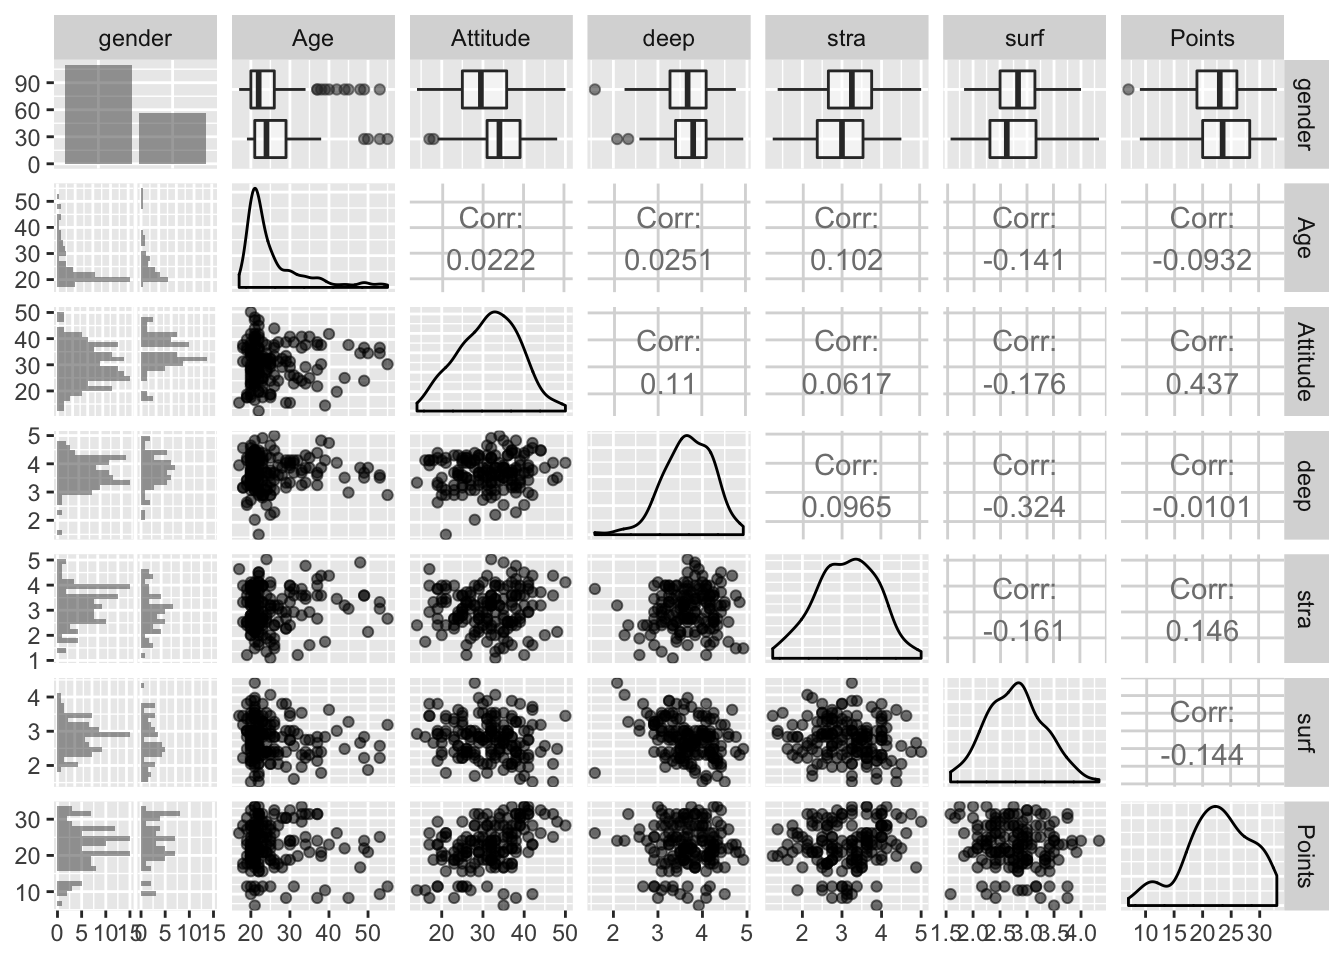
\includegraphics{chapter2_files/figure-latex/unnamed-chunk-7-1.pdf}
\includegraphics{chapter2_files/figure-latex/unnamed-chunk-7-2.pdf}
\includegraphics{chapter2_files/figure-latex/unnamed-chunk-7-3.pdf}

\hypertarget{residuals-vs-fitted-values}{%
\subsection{Residuals vs Fitted
values}\label{residuals-vs-fitted-values}}

This plot shows that the residuals have constant variance. You can find
an equally spread residuals around the horizontal line without distinct
patterns.

\hypertarget{q-q-plot-normality}{%
\subsection{Q-Q plot (normality)}\label{q-q-plot-normality}}

With the Q-Q plot you can explore that the residuals are normally
distributed. As you can see the points are very close to the line. There
are the upper and lower tails which have some deviation. I think this is
acceptable. I would interpret that the errors are normally distributed.

\hypertarget{residuals-vs-leverage}{%
\subsection{Residuals vs Leverage}\label{residuals-vs-leverage}}

This plot helps you to understand if there are outliers in the data that
are influencial in the linear regression model. In this analysis all the
cases are inside the Cook's distance lines.


\end{document}
